\textnormal{
The deliverables for this stage include the system flow diagram containing a graphical representation and textual descriptions of the corresponding data transformations, high level pseudo code of the overall system operation, and overall system time and space complexity.}

\begin{itemize}
\item{ }
Since the target of this project is an elaborate demonstration of A* algorithm in the form of "8-figure puzzle" game on a web site, the system should then be this web site. Distinct users, all regarded as game players, will enjoy playing the game along with viewing the process of implementing A* algorithm to solve the game, only that the advanced game players are qualified to control the visualization mode and speed.
\item{ }
Algorithms about web development and user interaction will not be discussed in this report. A* algorithm will be based on Javascript language and use data structures like array, hash table, priority queue,etc. The system design will also include an entity called "identity" recording the current user information and his authorization, will have attributes including "username", "password", "type", etc, and operations including "ChangePassword","Upgrade", etc, which help the system distinguish the user type and grant authorization accordingly.
\end{itemize}

Please insert your deliverables for Stage2 as follows:
\begin{itemize}
\item{  Short Textual Project Description. }
This project will be demonstrated in the form of a dynamic web site where canvas will be designed on the web page to make the visualization more attracting. The execution follow the flow of "home page-game page-visualization canvas-mode control", as shown more explicitly in figure 1.

The time complexity of A* depends on the heuristic. For the worst case of an unbounded search space, the number of nodes expanded is exponential in the depth of the solution d: $O(b^d)$, where b is the branching factor.

The space complexity of A* only is $O(n^2)$, the overall will vary with the web site status.

\item{ Flow Diagram. }
\begin{figure}[ht]
\centering
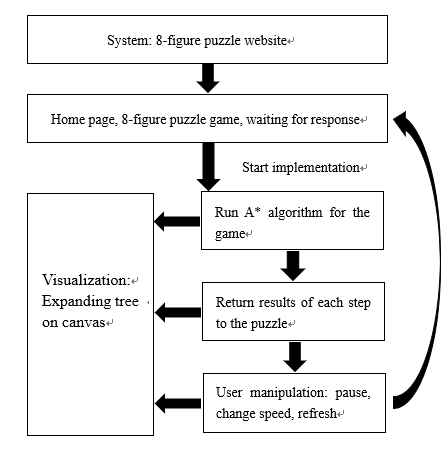
\includegraphics[width=3.13in]{figure1}
\label:{figure 1}
\end{figure}
Figure 1 indicates the execution diagram of the whole system, while the following figure 2 shows the flow diagram of A* algorithm.

\begin{figure}[ht]
\centering
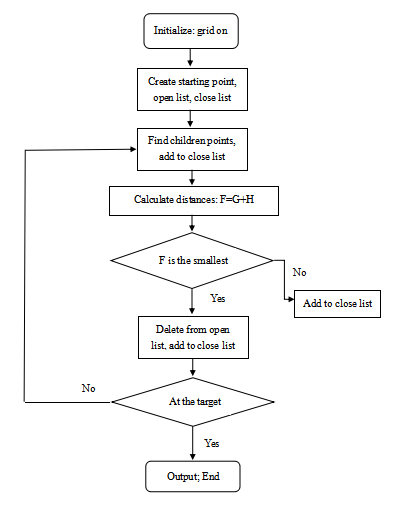
\includegraphics[width=3.5in]{figure2}
\label:{figure 2}
\end{figure}

\item{ High Level Pseudo Code System Description. }

\begin{lstlisting}[language={[ANSI]C}, title=pseudo code of A* algorithm, keywordstyle=\color{blue!70},
commentstyle=\color{red!50!green!50!blue!50},frame=shadowbox,rulesepcolor=\color{red!20!green!20!blue!20},
numbers=left,numberstyle=\tiny]
Astar(){
    Table open,close;
    inject(s,open);//s is the starting point
    while(open!=NULL){
        node n=ExtractMin(open);
        if(n==target){
            break;
        }
        for each x as child of n{
            if(x in open){
                if(cost(x)<cost(open)){
                    x.parent=n;
                    update(open);
                }
            }
            if(x in close){
                if(cost(x)<cost(close)){
                    x.parent=n;
                    update(close);
                    inject(x,open)
                }
            }
            else{
                x.parent=n;
                calculate cost(x);
                inject(x,open)
            }
        }
        inject(n,close);
        sort(open);
    }
    path p;
    for node x=target to s{
        p.generate(x)//starting from the target point and follows its parent node until the starting point
    }
    return p;
 }
\end{lstlisting}

\item{Algorithms and  Data Structures. }
The major algorithm is A* algorithm, which is a heuristic algorithm widely used in path finding and graph traversal. This project will use this algorithm to visualize the process of solving a "eight-figure puzzle" game.
The main data structures include array, hash table, priority queue, and probably object-oriented programming.
\end{itemize}

\begin{itemize}
\item{  Flow Diagram Major Constraints.}
Please insert here the integrity constraints:
\begin{itemize}
\item{ Integrity Constraint 1 }

Username, password: varchar(20), not replicable, not null

User type: one of "original", "advanced" and "administrator"
\end{itemize}
\begin{itemize}
\item{ Integrity Constraint 2 }

step speed: float number
\end{itemize}
\end{itemize}

